\section{}
\[
H(s)=\frac{1}{s}\,.
\]
\subsection{Bode-Diagramm}
\begin{center}
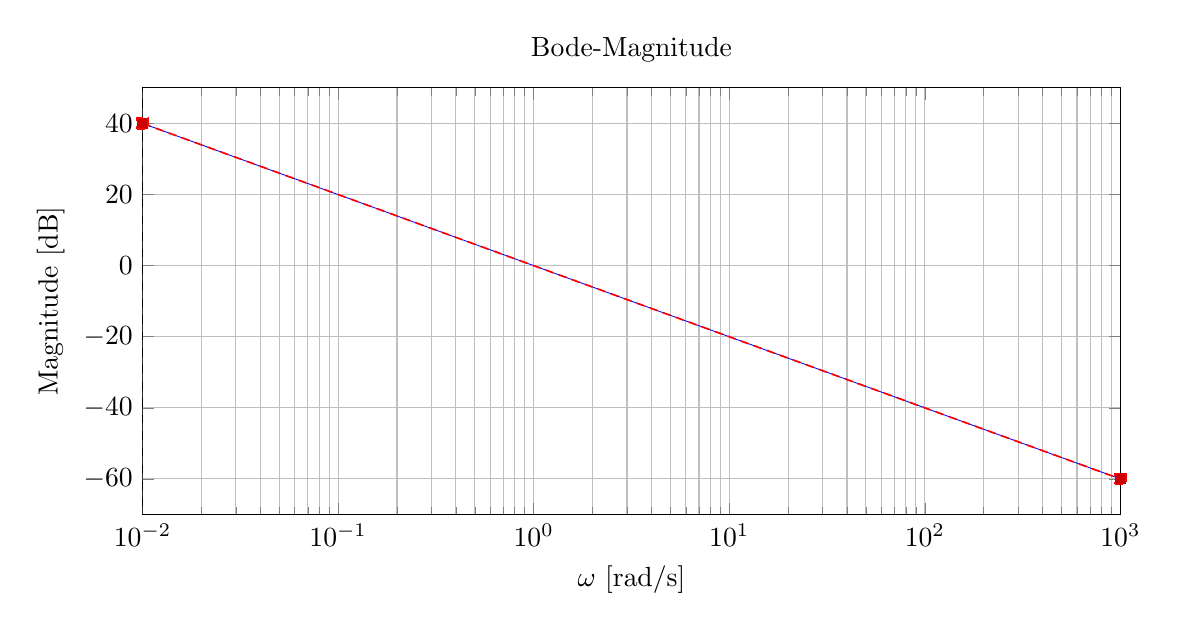
\begin{tikzpicture}
\begin{semilogxaxis}[
  width=14cm,height=7cm,
  ytick distance=20,
  xmin=1e-2,xmax=1e3,
  xlabel={$\omega$ [rad/s]},
  ylabel={Magnitude [dB]},
  grid=both,
  title={Bode-Magnitude}
]
\addplot[
  domain=1e-2:1e3,
  samples=400,
  mark=none,
  line width=0.3pt,
  blue
] {-20*ln(x)/ln(10)};
\addplot+[domain=1e-2:1e3,samples=2,dashed,dash pattern=on 3pt off 2pt,line width=0.6pt,red] {-20*ln(x)/ln(10)};
\draw[gray,dashed] (rel axis cs:0,0) -- (rel axis cs:0,1);
\end{semilogxaxis}
\end{tikzpicture}
\vspace{6mm}
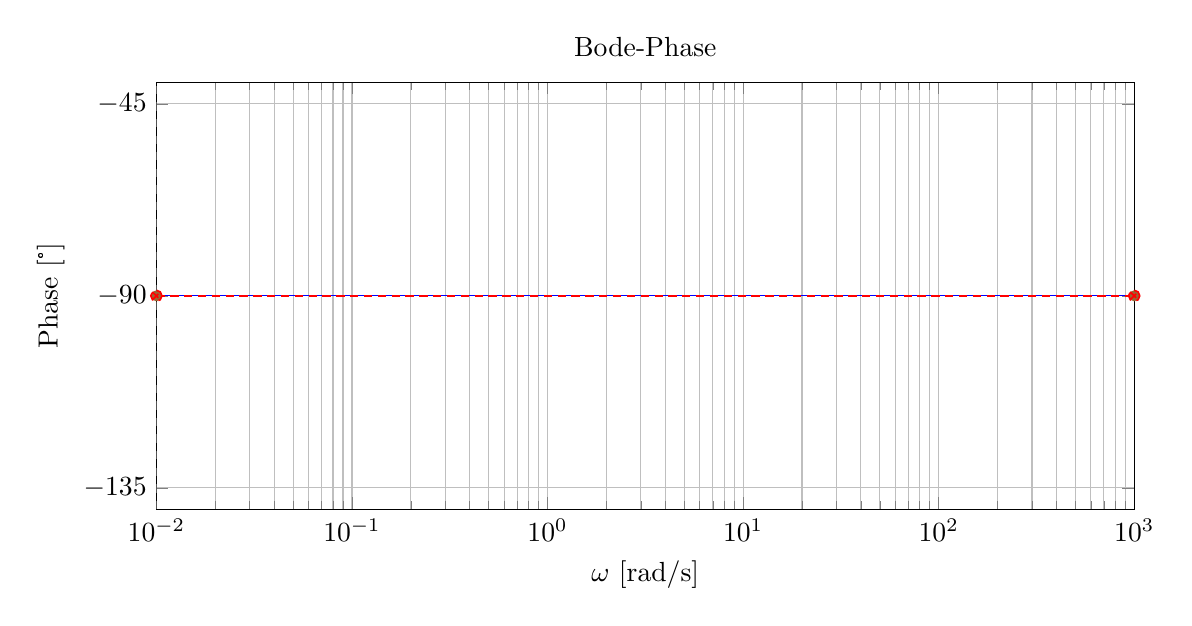
\begin{tikzpicture}
\begin{semilogxaxis}[
  width=14cm,height=7cm,
  xmin=1e-2,xmax=1e3,
  ymin=-140,ymax=-40,
  ytick distance=45,
  xlabel={$\omega$ [rad/s]},
  ylabel={Phase [°]},
  grid=both,
  title={Bode-Phase}
]
\addplot[
  domain=1e-2:1e-3,
  samples=2,
  mark=none,
  line width=0.3pt,
  blue
] {-90};
\addplot[
  domain=1e-3:1e3,
  samples=2,
  mark=none,
  line width=0.3pt,
  blue
] {-90};
\addplot+[domain=1e-2:1e3,samples=2,dashed,dash pattern=on 3pt off 2pt,line width=0.6pt,red] {-90};
\draw[gray,dashed] (rel axis cs:0,0) -- (rel axis cs:0,1);
\end{semilogxaxis}
\end{tikzpicture}
\end{center}
\newpage
\subsection{Erklärung (ausführlich)}
\begin{description}[leftmargin=1.2em,labelsep=.6em,font=\bfseries]

\item[1. Normalform herstellen.]
\[
H(s)=\frac{1}{s}=K_0\cdot s^{\,r},\qquad
K_0=1,\quad r=-1.
\]


\item[2. Eckfrequenzen bestimmen und sortieren.]
Keine endliche Eckfrequenz; nur Ursprungspol.

\item[3. Startpunkt des Amplitudengangs festlegen (Geradennäherung).]
Wähle Referenz \(\omega_{\mathrm{ref}}=1\,\mathrm{rad/s}\) (Fixpunkt).
\[
F_{\mathrm{dB}}(\omega_{\mathrm{ref}})=20\log_{10}\!\big(|K_0|\ \omega_{\mathrm{ref}}^{\,r}\big)
=20\log_{10}(1^{\,{-1}})=0\,\mathrm{dB}.
\]
Ankerpunkt: \(0\,\mathrm{dB}\) bei \(\omega=1\).

\item[4. Verlauf links vom Startpunkt zeichnen.]
Konstante Steigung \(r\cdot 20\,\mathrm{dB/dec} =-20\,\mathrm{dB/dec}\) über alle Frequenzen. Gerade durch den Ankerpunkt mit Steigung \(-20\,\mathrm{dB/dec}\).

\item[5. Steigungswechsel an den Eckfrequenzen eintragen.]
Kein Steigungswechsel (keine endliche Ecke).

\item[6. Eckabrundung korrekt berücksichtigen.]
Keine Ecken \(\Rightarrow\) keine \(\pm 3/6/9\,\mathrm{dB}\)-Korrekturen.

\item[7. Phasenstartwert festlegen.]
Da \(K_0\,F^*_{\mathrm{ges}}(0)>0\) und \(r=-1\):
\[
\varphi(0)=r\cdot 90^\circ = -90^\circ.
\]

\item[8. Phasenänderung durch Teilglieder eintragen.]
Nur Ursprungspol: Phase konstant \(-90^\circ\). Keine Überlappung, keine Addition weiterer Beiträge.

\item[9. Grenzwerte und Konsistenz prüfen.]
DC: \(|H(0)|\to\infty\Rightarrow +\infty\,\mathrm{dB}\), \(\varphi(0)=-90^\circ\).
HF: \(|H(j\omega)|=1/\omega\Rightarrow -20\log_{10}\omega\,\mathrm{dB}\), \(\varphi(\infty)=-90^\circ\).

\end{description}

\subsubsection*{Stückweise Näherungen (für die Skizze)}
\[
|H(j\omega)|_{\mathrm{dB}}\approx
\begin{cases}
-20\log_{10}\omega,& \omega\ll 1,\\[2pt]
0,& \omega=1,\\[2pt]
-20\log_{10}\omega,& \omega\gg 1,
\end{cases}
\]\[
\varphi(\omega)\approx -90^\circ\ \text{(für alle }\omega\text{)}.
\]

\newpage